\section{Grand Unification and SUSY}

\begin{frame}{Gauge Couplings in the Standard Model}
\addtocounter{framenumber}{-1}
The Standard Model is described as the most general renormalizable 	field theory with gauge group 
\begin{equation*}
	\mathcal{G}_{\mathrm{SM}} = \mathrm{SU}(3) \times \mathrm{SU}(2) \times \mathrm{U}(1),
\end{equation*}
with  associated gauge couplings $\alpha_3$, $\alpha_2$ and $\alpha_1$,
three generations of fermions and a scalar \cite{Hebecker2020}. \\[2em]
\begin{itemize}
\item The couplings are larger for the larger component of the gauge group, i.\,e. \begin{equation*}
	\alpha_3(m_Z) > \alpha_2(m_Z) > \alpha_1(m_Z)
	\end{equation*}
	\item Interesting observation: Values of the running couplings come close together at some high energy scale $\Lambda_{\mathrm{GUT}} \sim 10^{16}\ \mathrm{GeV}$ (cf. next slide).\\[1em]
	\item \alert{\textsc{Georgi-Glashow}} \cite{GeorgiGlashow1974}: Embed $\mathcal{G}_{\mathrm{SM}}$ in larger gauge group, i.\,e. $\operatorname{SU}(5) \implies \mathrm{GUT?}$  
 \end{itemize}
 \end{frame}

\begin{frame}{One Loop Running of the SM Gauge Couplings I}
	\begin{figure}
	\centering
	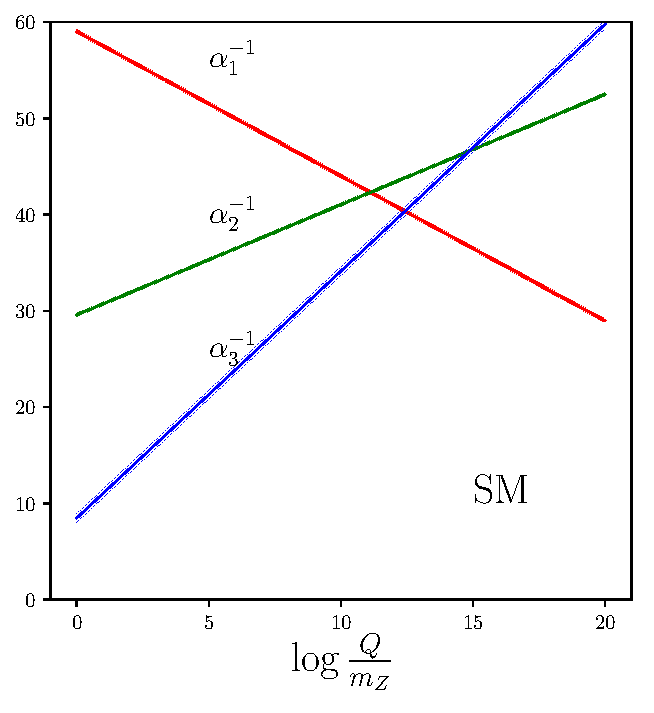
\includegraphics[scale = 0.6]{figures/dgut-1}%\hspace{3em}
	\caption{Running of the (inverse) SM gauge couplings, plot inspired by \cite{Kazakov2000}.}
	\end{figure}
\end{frame}

\begin{frame}{One Loop Running of the SM Gauge Couplings II}
	\begin{itemize}
			\item In the Georgi-Glashow model, we need $-\mu^2 \sim -(100\ \mathrm{GeV})^2$ to reproduce the correct $W$ and $Z$ masses $\implies$ \alert{Gauge hierarchy problem!} \cite{PeskinSchroeder1995}\\[1em]
		\item SUSY provides way out: If SUSY breaking works such that the mass differences between the superpartners are large enough, one can reproduce the correct Higgs mass $\implies$ superpartners influence the running of the (MS)SM gauge couplings (cf. next slide)
	\end{itemize}
\begin{figure}
	\centering
	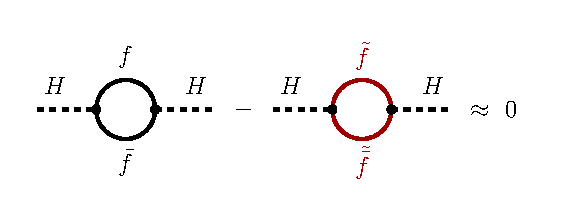
\includegraphics{figures/running_diagrams.pdf}
	\begin{itemize}
		\item In the end it remains a complicated \alert{fine tuning} task!
	\end{itemize}

	\end{figure}	

\end{frame}


\begin{frame}{Comparison: SM vs. MSSM}
	\begin{figure}
	\begin{subfigure}
		\centering
	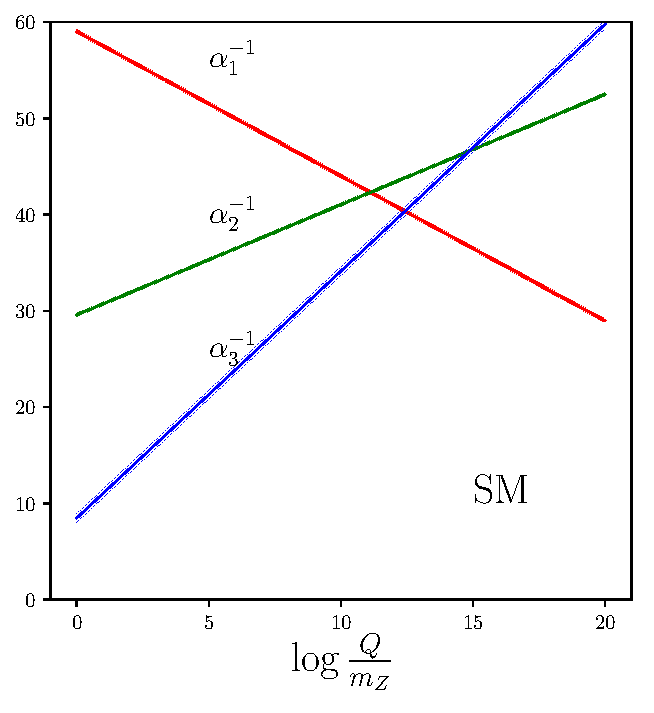
\includegraphics[scale = 0.55]{figures/dgut-1}
	\end{subfigure}
	\begin{subfigure}
		\centering
	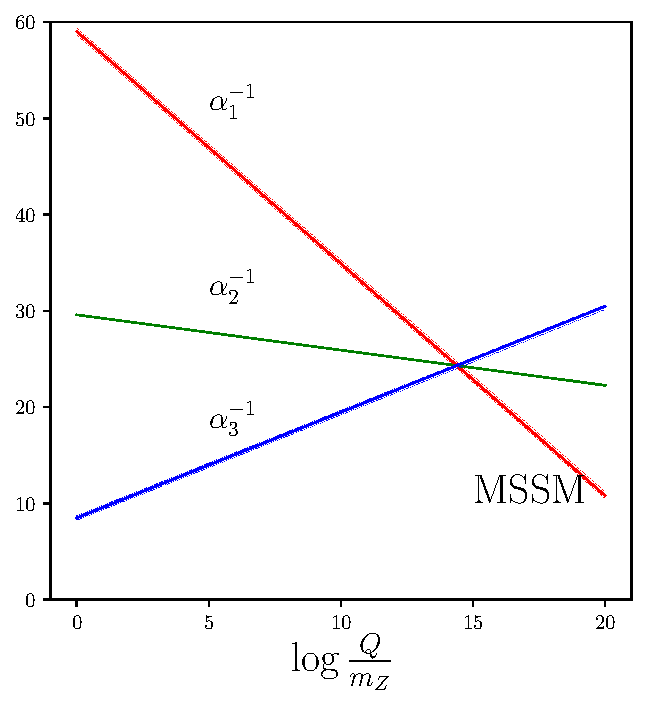
\includegraphics[scale = 0.55]{figures/dgut-2}
	\end{subfigure}

	\caption{Running of the (inverse) gauge couplings in the SM and the MSSM, plots inspired by \cite{Kazakov2000}.}
	\end{figure}
\end{frame}

